\gobbletocpage
\chapter{Introduction}
\restoretocpage

%\pagestyle{chapter}
\begin{shadequote}
The sure and definite determination (of species of bacteria) requires so much time, so much acumen of eye and judgement, so much of perseverance and patience that there is hardly anything else so \mbox{difficult}. \par--\emph{Otto F. M\"uller}
\end{shadequote}

\section{Description of Problem}
The quote above, by no mistake, graced the cover of the International Journal of Systematic and Evolutionary Microbiology for decades.
Whereas plant and animal systematists are guided by a theory-based approach to demarcating species, microbiologists have yet to agree on a set of ecological and evolutionary properties that could serve to identify bacterial species~\cite{cohan2007systematics}.
Microbiologists are naturally handicapped by the paucity of morphological differences that could aid in differentiation of closely related bacterial species.
Additionally microbiologists cannot predict which traits will cause a speciation event since bacteria are capable of receiving genes from distant relatives through a process known as horizontal gene transfer (HGT)~\cite{cohan2007systematics}.
%Thus, in order to effectively understand the microbiome we must strive towards developing a method for consistently demarcating groups, from bacterial diversity, that play distinct ecological roles~\cite{koeppel2008identifying}.
Thus, in order to effectively understand the inherent intricacy of the microbiome we must strive towards developing a method for consistently demarcating groups of bacteria that play distinct ecological roles~\cite{koeppel2008identifying}.

Initially, closely-related bacterial species were identified based on metabolic phenotype traits.
Systematists now rely on molecular approaches that utilize the decreasing cost of DNA sequencing to compare genetic information.
A 70\% cutoff was established for whole genome hybridization studies (comparing loss and gain of large segments of DNA), replaced by varying degrees of sequence identities in homologous genes~\cite{cohan2007systematics,carlo,staley1997biodiversity}.
Building on these technological breakthroughs microbiologists have taken great steps towards understanding bacteria speciation, yet they have brought into focus new difficulties.

\subsection{Diversity of Bacterial Species}
Modern molecular techniques have revealed an extraordinary diversity of microorganisms, most of which are as yet uncharacterized~\cite{bohannan2003new}.
Estimates of eukaryotic diversity fall within the range of 10 to 50 million species~\cite{may1988many}. Even though we have only observed approximately 9000 prokaryotic species, indirect approaches that do not rely on cultivation hint towards the existence of a billion or more prokaryotic species worldwide ~\cite{dykhuizen1998santa} and \textasciitilde10 million within a given habitat~\cite{gans2005computational}.
To observe biodiversity through molecular means, scientists should find organisms in highly distinct sequence clusters; since each cluster has had a long history of separate evolution they have likely evolved unique adaptations shared by the entire cluster~\cite{cohan2007systematics}.
The only rational approach to clustering such a large group of diverse organisms effectively is with a theory based molecular method that can be standardized and applied to large numbers of sequences.

Current protocols for deciding bacterial lineages are functionally inadequate.
Recent ecological studies demonstrate that a named bacterial species is typically an assemblage of closely related but ecologically distinct populations~\cite{cohan2007systematics}.
Thus, within a named species established by antiquated methods, one may find distantly related organisms that do not naturally fit in with what we will define to be a cohesive species cluster, thus contradicting ideal approaches to understanding and cataloguing biodiversity.
Through such an inadequate and archaic system comprehensive study becomes impossible.

Fortunately for microbiologists organisms from every known community appear to cluster into discrete ecologically interchangeable individuals~\cite{cohan2007systematics}.
Clustering is a universal feature at all levels of diversity, owning to different rates of survival and extinction~\cite{darwin1861origin}.
Our envisioned demarcation algorithm would be capable of identifying putative clusters of ecologically distinct organisms within named bacterial clades.
While accuracy is of utmost importance, due to the large numbers of potential bacterial species we would appreciate an efficient demarcation algorithm.

\begin{figure}
\centering
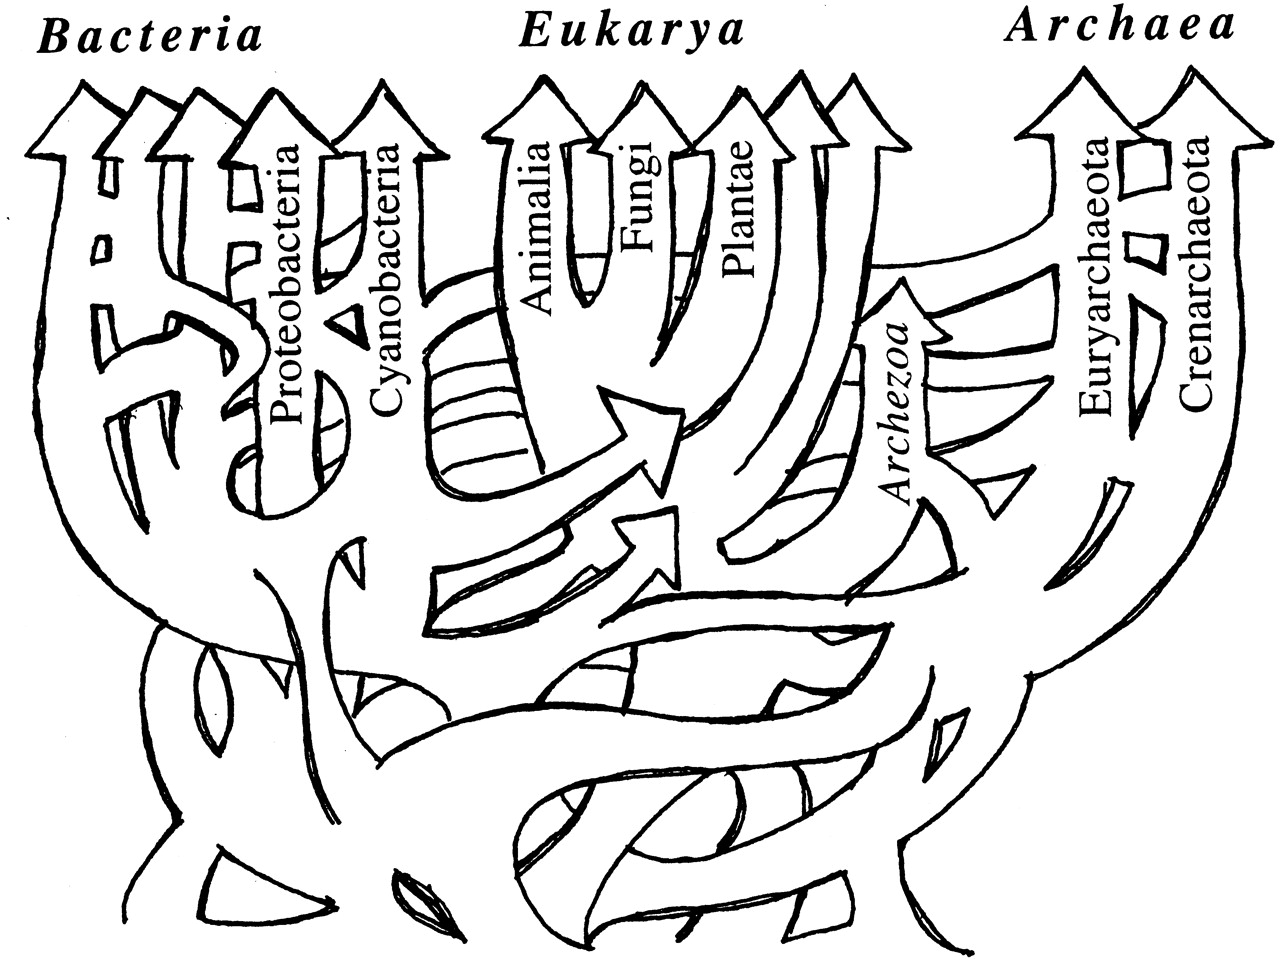
\includegraphics[scale=0.25]{images/HGTTree-CH1}
\label{fig:HGTmodel}
\caption[Model tree representing HGT.]{Model tree representing HGT. The arrows represent genetic exchange between lineages. Notice how genetic material is also shared across kingdoms. (reprinted from\protect\cite{doolittle1999phylogenetic}).}
\label{fig:HGTmodel}
\end{figure}

\subsection{Differences of Bacterial Population Dynamics}
As briefly mentioned earlier there exist peculiarities of bacterial population dynamics that complicate demarcation.
These characteristics are important to keep in mind when thinking about approaches to bacterial species demarcation.

\subsubsection*{Asexual reproduction}
Prokaryotes have the ability to reproduce clonally.
In fact, genetic exchange occurs typically through processes not tied to reproduction.
Because of low level frequencies of genetic exchange, sexual isolation is not a pre-requisite for permanent divergence between distinct ecological bacterial populations ~\cite{cohan2007systematics}.
This means that sympatric speciation becomes a common occurrence.
Early models for understanding adaptation, evolution, and speciation in these organisms often focus on clonality and periodic selection~\cite{gogarten2002prokaryotic}.
Genetic exchange plays a different role in evolution from that of plants and animals; it is assessed to be very rare and when it occurs only short segments can be successfully transferred.
Also, mutations in haploid bacteria will immediately be phenotypically expressed, resulting in rapid displacement of a parental genotype~\cite{staley1997biodiversity}, changing the dynamics of speciation.

\subsubsection*{Horizontal Gene Transfer (HGT)}
When genetic exchange does occur, in contrast to eukaryotes, bacterial genetic features can be transferred among distantly related bacteria via various genetic exchange mechanisms such as transformation and conjugation.
Genetic features may reside in the cell, on a plasmid, or become incorporated into the bacterial chromosome~\cite{staley1997biodiversity}.
HGT even can occur between very distantly related organisms e.g., between bacteria and plants or fungi~\cite{gogarten2002prokaryotic} (see Figure~\ref{fig:HGTmodel} on page~\pageref{fig:HGTmodel}).
It leads to genomes whose constituent genes have different evolutionary histories~\cite{gogarten2002prokaryotic} and can thus complicate the species identification process.


\section{Demarcation Software}
Today there are several freely distributed demarcation programs available: Ecotype Simulation (ES1), BAPS, GMYC, AdaptML, and newly introduced Ecotype Simulation 2 (ES2), which is an improvement on ES1.
Each is an attempt to define species as a fundamental unit, usable in practical applications a few of which I will highlight in the following section.
They all differ in background theory, resulting in different demarcations.
I will focus specifically on ES1 and the improvements resulting in ES2 which are both ecotype-based systematics proposed for identifying ecotypes, the fundamental units of bacterial ecology and evolution.
Ecotypes are ecologically distinct from each other, and each has homogenous membership~\cite{cohan2007systematics}.
More details about ecotypes will be in following chapters.

Most people are interested in direct practical applications.
Programming simulation software and bacterial speciation software, one often tends to forget about real-world applications.
The benefits of working somewhere that has a wet-lab component is that it allows researchers to focus on the theoretical and applied.

\section{Practical Applications}
We must first be able to identify the basic units operating within the system in order to understand the microbiome.
Once we have established the atomic functional unit we can then start building collections of relationships between these units.
With an understanding of microbial population dynamics comes positive real world applications.

\subsubsection*{Anticipation of future human pathogens}
Preparing for future epidemics, we should try and discover all long-standing ecotype diversity within each named pathogenic species, allowing us to anticipate disease-causing properties of each ecotype~\cite{cohan2007systematics}.
There is a large and diverse microbiome within every living organism's gut.
Many believe that certain diseases are caused by imbalances in normal microbial fauna~\cite{ballal2011host}.
We are not far from the day where we could analyze an individual's gut ecosystem and predict afflictions.

\subsubsection*{Biotechnology}
After discovering a strain with a valuable enzyme, one could then search for homologs in each ecotype closely related to the strain, potentially allowing discovery of similar enzymes with different substrates or with optima at different conditions~\cite{cohan2007systematics}.
This is particularly a useful concept for developing improved biofuel producing bacteria.
Microbial fuel cells hold great promise as a sustainable biotechnological solution to future energy needs, however current efforts to improve the efficiency of such fuel cells are limited by the lack of knowledge about the microbial ecology of these ecosystems~\cite{rabaey2004biofuel}.
Demarcation algorithms help research microbial systems, eventually uncovering beneficial pathways that the biotechnology industry can take advantage of.
However, more knowledge is necessary.
Improved biocatalysts and cellulase preparations are the major technical roadblocks to building a successful bioethanol industry~\cite{dien2003bacteria}.
Improvements in bacterial speciation understanding could save billions of dollars by uncovering more efficient ways of producing biofuels.

\subsubsection*{Simplify the burden of industrial testing of bacterial strains for their safety and efficacy in agricultural applications}
For example, for any named species that is heterogeneous for characteristics of safety concern (such as secreted metabolites and persistence in the environment) the European Union requires that any new strain developed for release be tested for these characteristics of concern.
However, individual strains from a species known to be homogeneous for these features need not be tested, thus demarcating taxa as ecologically homogeneous units would obviate or at least lessen the burden of these tests~\cite{cohan2007systematics}.
Dealing with microbial strains can be difficult and costly, however utilizing a theory-based demarcation algorithm for bacterial identification and comparison could reduce those costs as is generally the case through standardization.

\subsubsection*{Bioremediation}
Bioremediation has the potential to restore contaminated environments inexpensively yet effectively, but a lack of information regarding the factors controlling growth and metabolism of microorganisms in polluted environments regularly limits its implementation~\cite{lovley2003cleaning}.
Demarcation algorithms could be an invaluable step in the search for microbial bioremediation tools.
If we find a gene with a positive property in one ecotype, using a theory based speciation concept, we could quantitatively look for similar ecotypes, hypothesizing the availability of similar genes.
Combining models that can predict the activity of microorganisms that are involved in bioremediation with existing geochemical and hydrological models should transform bioremediation from a largely experimental practice into an industry standard program~\cite{lovley2003cleaning}.
Once again, much positive change could be brought about through the intelligent use of microbe interactions.

\subsubsection*{True quantification of ecological diversity within a community}
In the more theoretical realm, microbial ecologists are often interested in the factors that regulate community diversity across temporal and spatial scales; the impact of human activities on this diversity and the consequences of this diversity for ecosystem processes~\cite{bohannan2003new}.
Identifying taxa at the level of ecotypes, systematics will allow microbiologists to optimize their choice of sequencing targets, because from a sample one can determine how representative it is of the environment~\cite{bohannan2003new}.
This would allow researches to gain a more comprehensive perception regarding the larger microbial ecosystem for each habitat.
%More easily giving us an idea of a microbial ecosystems species content.
%Ideally, one should choose organisms from different ecotypes to get a fuller gene content survey of the ecosystem~\cite{cohan2007systematics}.
As mentioned briefly before, current methods for surveying diversity involves binning and assigning an operational taxonomic unit without a theoretical justification.

Ecotype demarcation will allow quantification of the ecological diversity within a community; a step toward understanding the plethora of ecological interactions within natural microbial communities~\cite{cohan2007systematics}.
Such information would provide researchers and industries more accurate and objective knowledge regarding the speciation of fundamental bacterial units; on the path to understanding complex microbial ecosystem's intrinsic value.


\section{Outline}
%My aims for this project are several.
I have many goals for this project, of which the final result should be a production-ready version of the optimized Ecotype Simulation (ES2) software.
However, first we plan on carrying out several tests to confirm if ES2 is accurate, and efficient in demarcating bacterial species.
I will run ES2 through the same test parameters the Cohan lab used to test ES1 against all available demarcation algorithms~\cite{carlo}; including generated datasets and environment collected sequences.
%It is important to demonstrate similar accuracy scores of ES2 to ES1.
We hypothesize that the new, more efficient, demarcating algorithm within ES2 will not significantly affect the accuracy of our output.
%Next, I want to identify the new reasonable upper limit for input size (i.e., number of sequences) for ES2.
Then I will run ES2 in conjunction with other available demarcation programs (BAPS, GMYC, AdaptML) on large generated datasets (up to the limit of our input generator) and evaluate demarcation accuracy and speed.

Chapter 1 introduced the problem that ES tries to address, and the benefits that understanding bacterial speciation will achieve.
The following chapter will go over several molecular models for bacteria speciation, their underlying algorithms, and their design and implementation in ES.
The next section discusses our approach to ES optimization and differences in ES2.
Chapter 4 will compare results of the various programs regarding demarcation speed and accuracy.
Finally, the conclusion will contain a discussion of the entire project, a section about work on future improvements, and concluding remarks.

